Come richiesto dalle specifiche funzionali,
il sistema implementato fornisce un'interfaccia che permette di
scegliere in fase di inizializzazione la mappa statica totale
e il numero di robot da collocarvi.

Per quanto riguarda la verifica della
\emph{correttezza del risultato},
viene fornita una visualizzazione complessiva del luogo raccogliendo
informazioni centralizzate unicamente volte a controllare
l'esecuzione del sistema.
L'utente può in questo modo controllare che il risultato del
sistema sia coerente con le specifiche definite in Sezione~\ref{sec:func-req},
in base all'attuale posizione dei robot.
In quanto la posizione e il movimento di questi ultimi è variabile,
non è stato possibile allegare insiemi di test che potessero
riguardare il risultato di un singolo tentativo di una query.
Sono invece allegati al progetto una serie di grafi generali
e di relative query per cui il risultato atteso può essere verificato
possibilmente dopo alcuni tentativi successivi (risultanti
in \texttt{DONTKNOW}) della stessa query.
Per facilitare questa fase, è stata inserita l'opzione \emph{auto-move-and-retry} che ritenta la query dopo aver fatto muovere i robot
in modo automatico fino al raggiungimento di un
\texttt{MATCH} o \texttt{FAIL}.

\begin{figure}
\centering
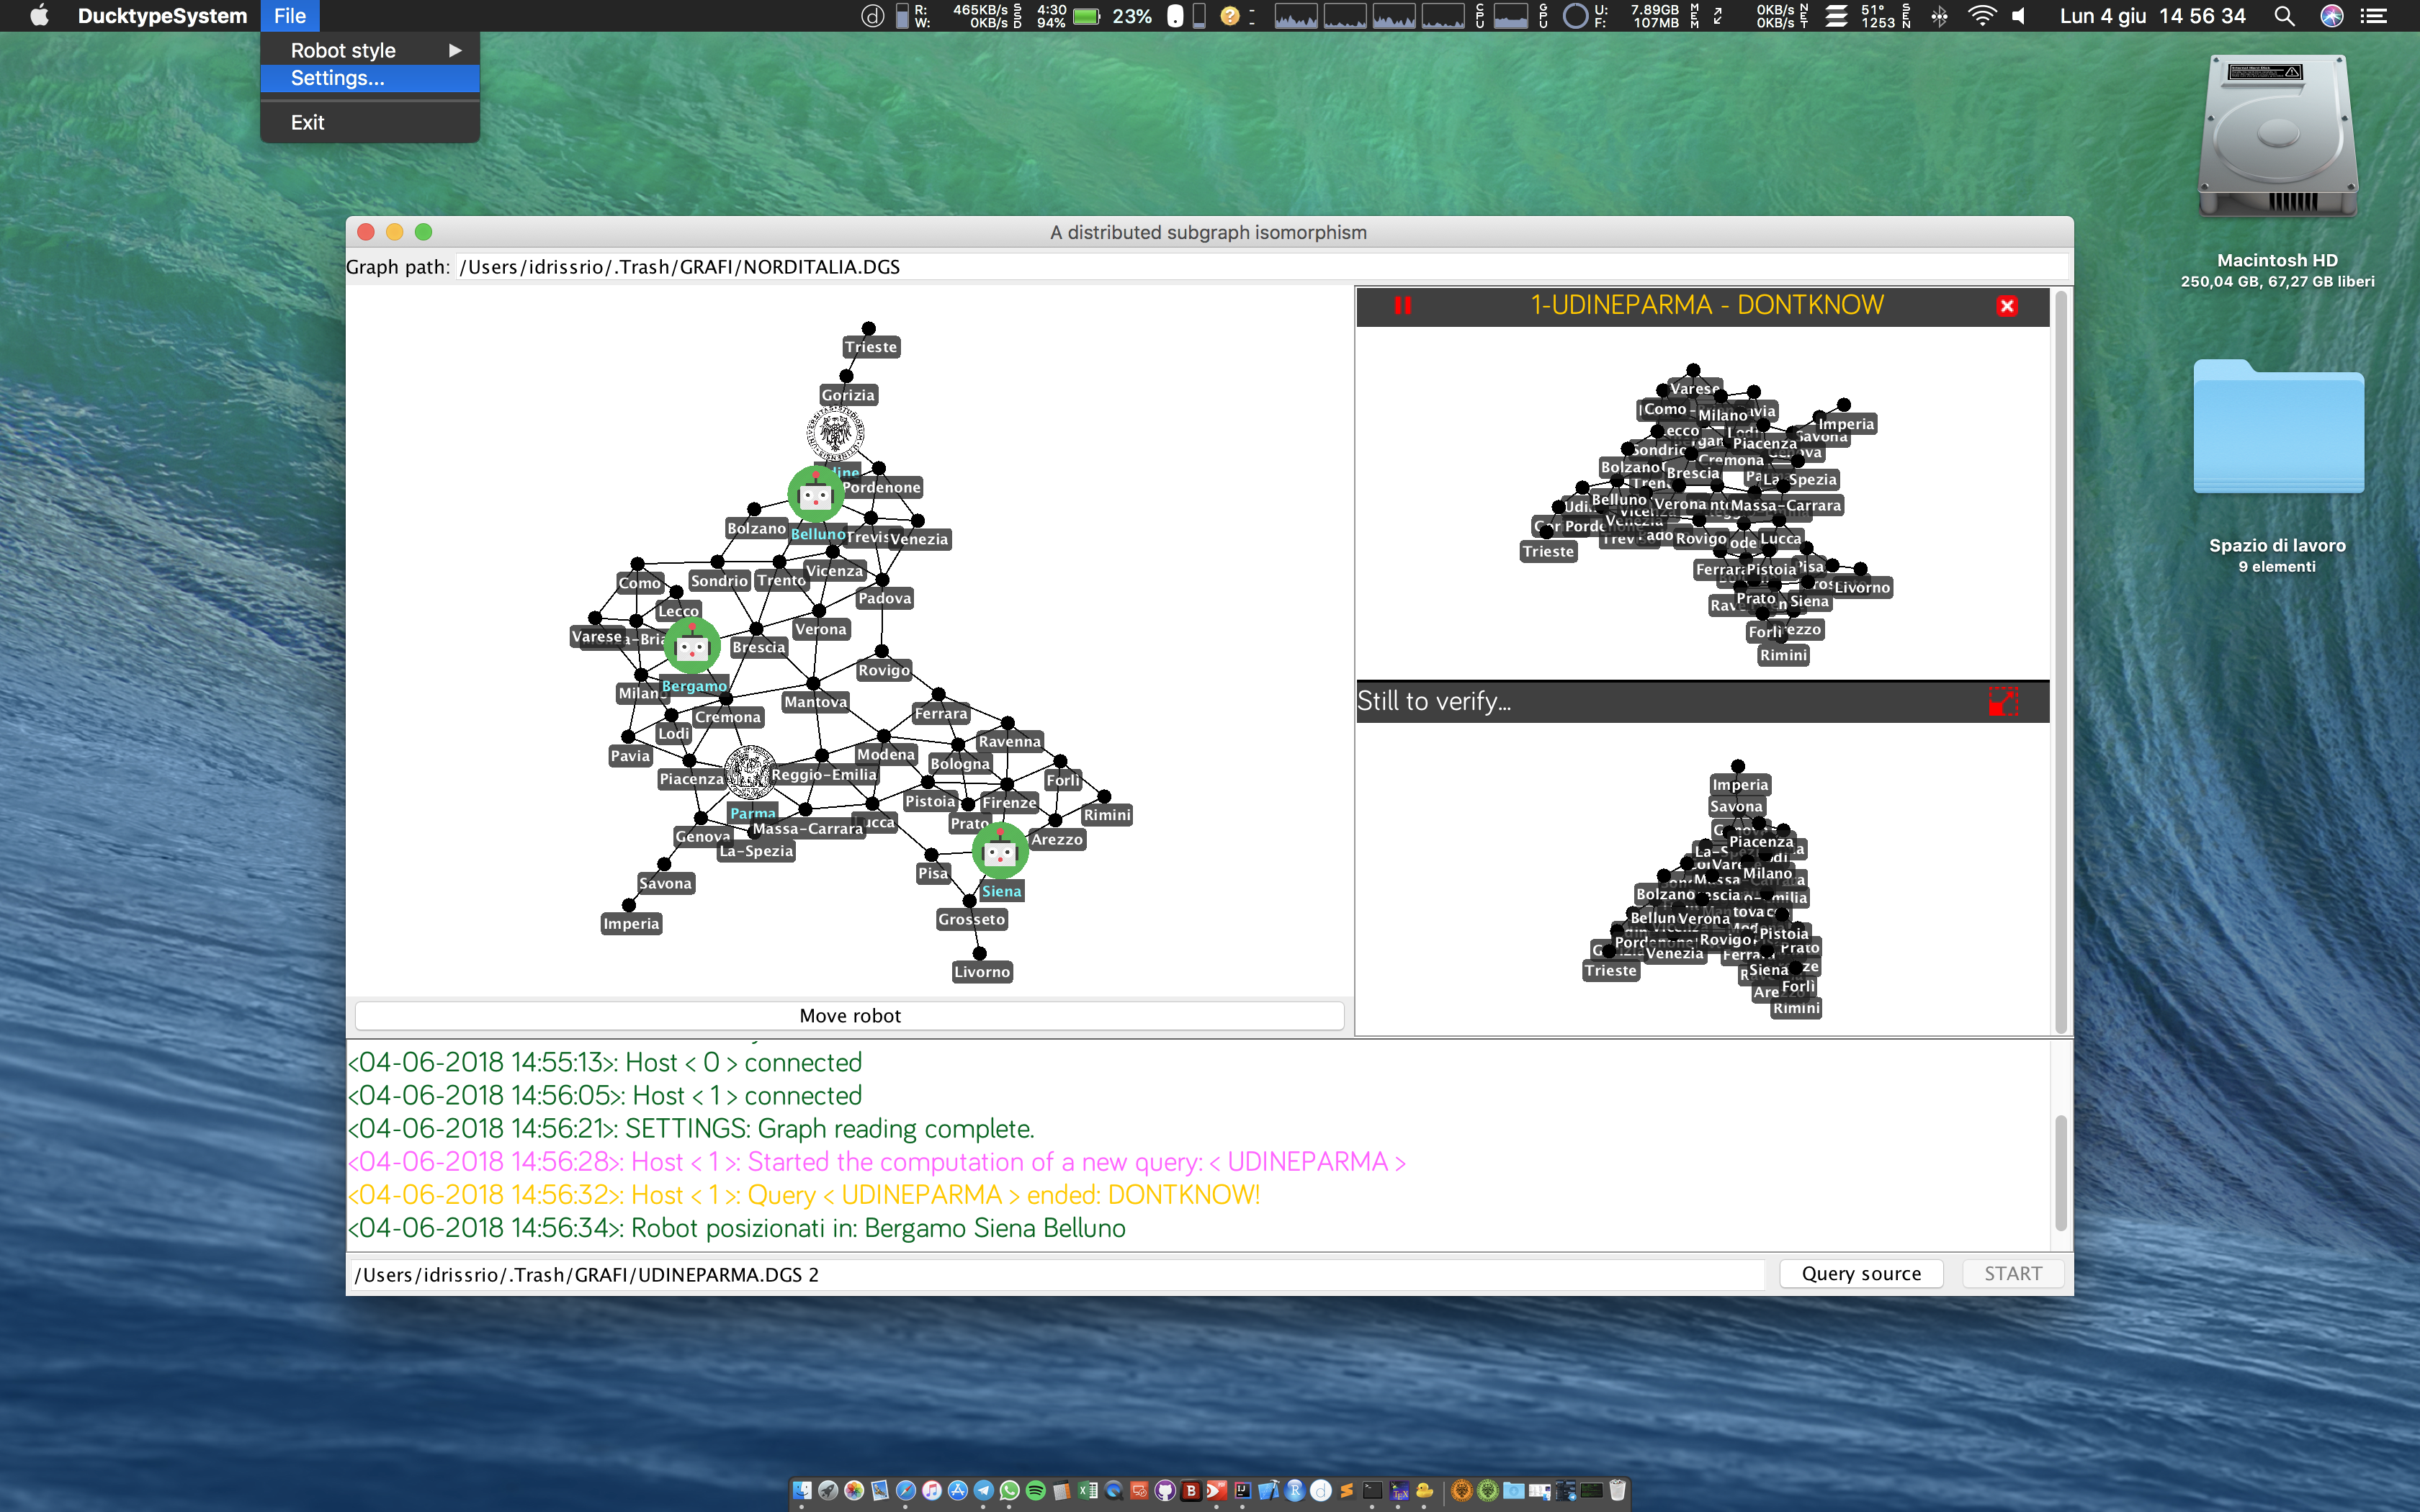
\includegraphics[width=1\textwidth]{immagini/inizioQuery.png}
\caption{La view principale descritta nella Sezione \ref{sec:viewImpl}.
In basso il log di sistema. A sinistra la visualizzazione dello stato di ogni query.
Nel centro la topologia del grafo principale.}
\end{figure}
\begin{figure}
\centering
\includegraphics[width=1\textwidth]{immagini/betterVisualization.png}
\caption{Modalità \emph{better visualization}: essendo
alcuni grafi molto grandi, è stata introdotta la possibilità di
scorporare il \emph{JPanel} di destra in una finestra a sè
stante, permettendo una migliore visualizzazione delle query.}
\end{figure}

Le caratteristiche non funzionali descritte nella Sezione~\ref{sec:nonfunc-req}
possono essere validate osservando la struttura del progetto.
Mentre la scalabilità e la location transparency vengono ereditate
principalmente da \emph{Akka},
il grado di fault tollerance offerto è dato da interventi \emph{ad-hoc}
sul nostro codice: questo permette all'utente di verificare più
concretamente la resilienza del sistema al presentarsi dei
particolari fallimenti presi in considerazione.
I fallimenti dei processi (\emph{DSQueryChecker} e \emph{DSRobot})
sono stati infatti simulati esplicitamente nel codice,
e avvengono con una probabilità settabile tramite l'interfaccia grafica
del sistema, come mostrato in Figura~\ref{fig:settings}.
\begin{figure}
	\centering
	\includegraphics[width=0.5\textwidth]{immagini/settings.png}
	\caption{\label{fig:settings}
        Impostazioni di sistema utilizzate per simulare i fallimenti.}
\end{figure}
Impostando probabilità di fallimenti molto alte si potrà verificare
un considerevole aumento dei tempi di verifica di una query,
in quanto il sistema deve provvedere a sostituire alcuni processi
ed eventualmente a ricominciare la verifica di una query perduta in
fase critica.

Al fine di apprezzare e poter controllare al meglio l'esecuzione,
sono stati introdotti dei \emph{Thred.sleep()} nel codice,
che rallentassero alcune fasi. Per questo, aggiungendo numerosi robot
è possibile che i tempi di verifica aumentino considerevolmente.

L'esecuzione interna e i messaggi scambiati secondo il protocollo
definito sono interamente verificabili tramite la lettura del
log dei messaggi interni del sistema.
Una dettagliata spiegazione dei messaggi e su come fare a ottenere
il file di log è riportata nell'Appendice~\ref{sec:log-interni}.

